
\chapter{Test program}\label{chap:test}


The strength in dividing development of a program into layers is that each layer can be developed, debugged and tested individually. If all layers are working individually, putting them together should prove much easier. Each of the layers are therefore debugged and tested individually before the final application is created. To be able to make easy and similar tests for all the layers, it was decided to develop a program for testing. Though there are two different ways to test a layer, the methods are the same.

\section{Testing by substituting surrounding layers}
To make it easy to change and manipulate the input and output, is it defined in .dat documents. Therefore the program doesn't have to be changed for different input, and the output can be easily extracted for further analysis. \custtt{Ifstream} and \custtt{Ofstream} are used to read and write from the documents. 
As the boost buffer is used as communication between the layers, is it also used as the test functions mean of communication with the layer tested. There are defined four buffers, two for input and two for output.
Figure \ref{fig:Layer_inputoutput}

\begin{figure}[htb]
	\begin{center}
	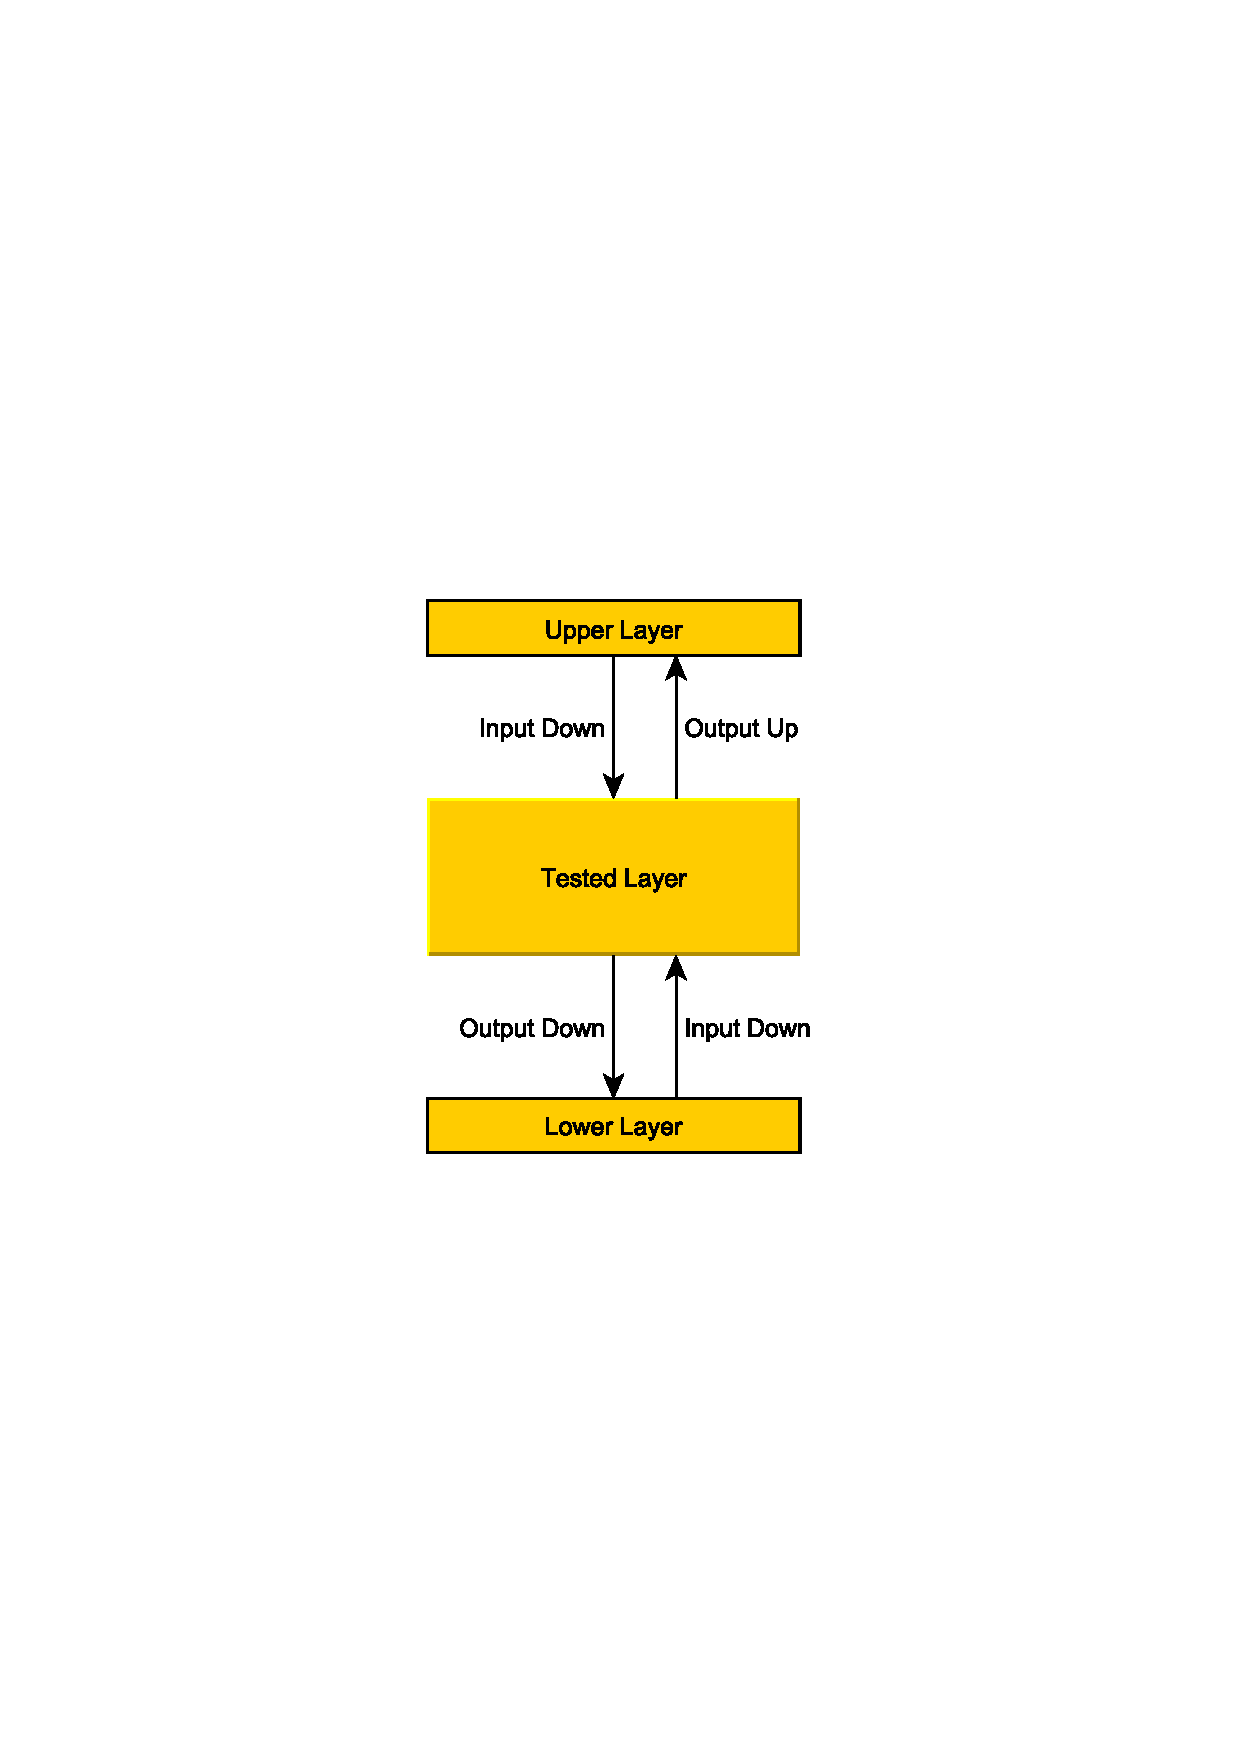
\includegraphics[scale=0.5,trim=0 200 0 200]{Layer_inputoutput.pdf}
	\caption{Substituting surrounding layers}
	\label{fig:Layer_inputoutput}	
	\end{center}
\end{figure}

\subsection{Testing a single instance of a layer}  

 The test program is able to send data to a layer as if it was the neighboring layers. Thus the program makes it possible to give input to a layer and check the output. This method is used to check if a layer is capable of  handling input and producing the expected output. This test is of course done throughout the development of the layers.


\subsection{Testing communication between two instances of a layer}

Another way to test a layer is to test actual communicating between two systems. In this test two instances of a layer is created, the upper layers are substituted as the single instance test. The lower layers are substituted with two buffers acting as respectively  input and output for the two layers as seen in Figure \ref{fig:twoInstanceTest}.The two instances can then communicate, as if the lower layers are working perfectly. This way it is possible to test if all the functions of a layer is working, when communicating with another instance of itself.




\begin{figure}[htb]
	\begin{center}
	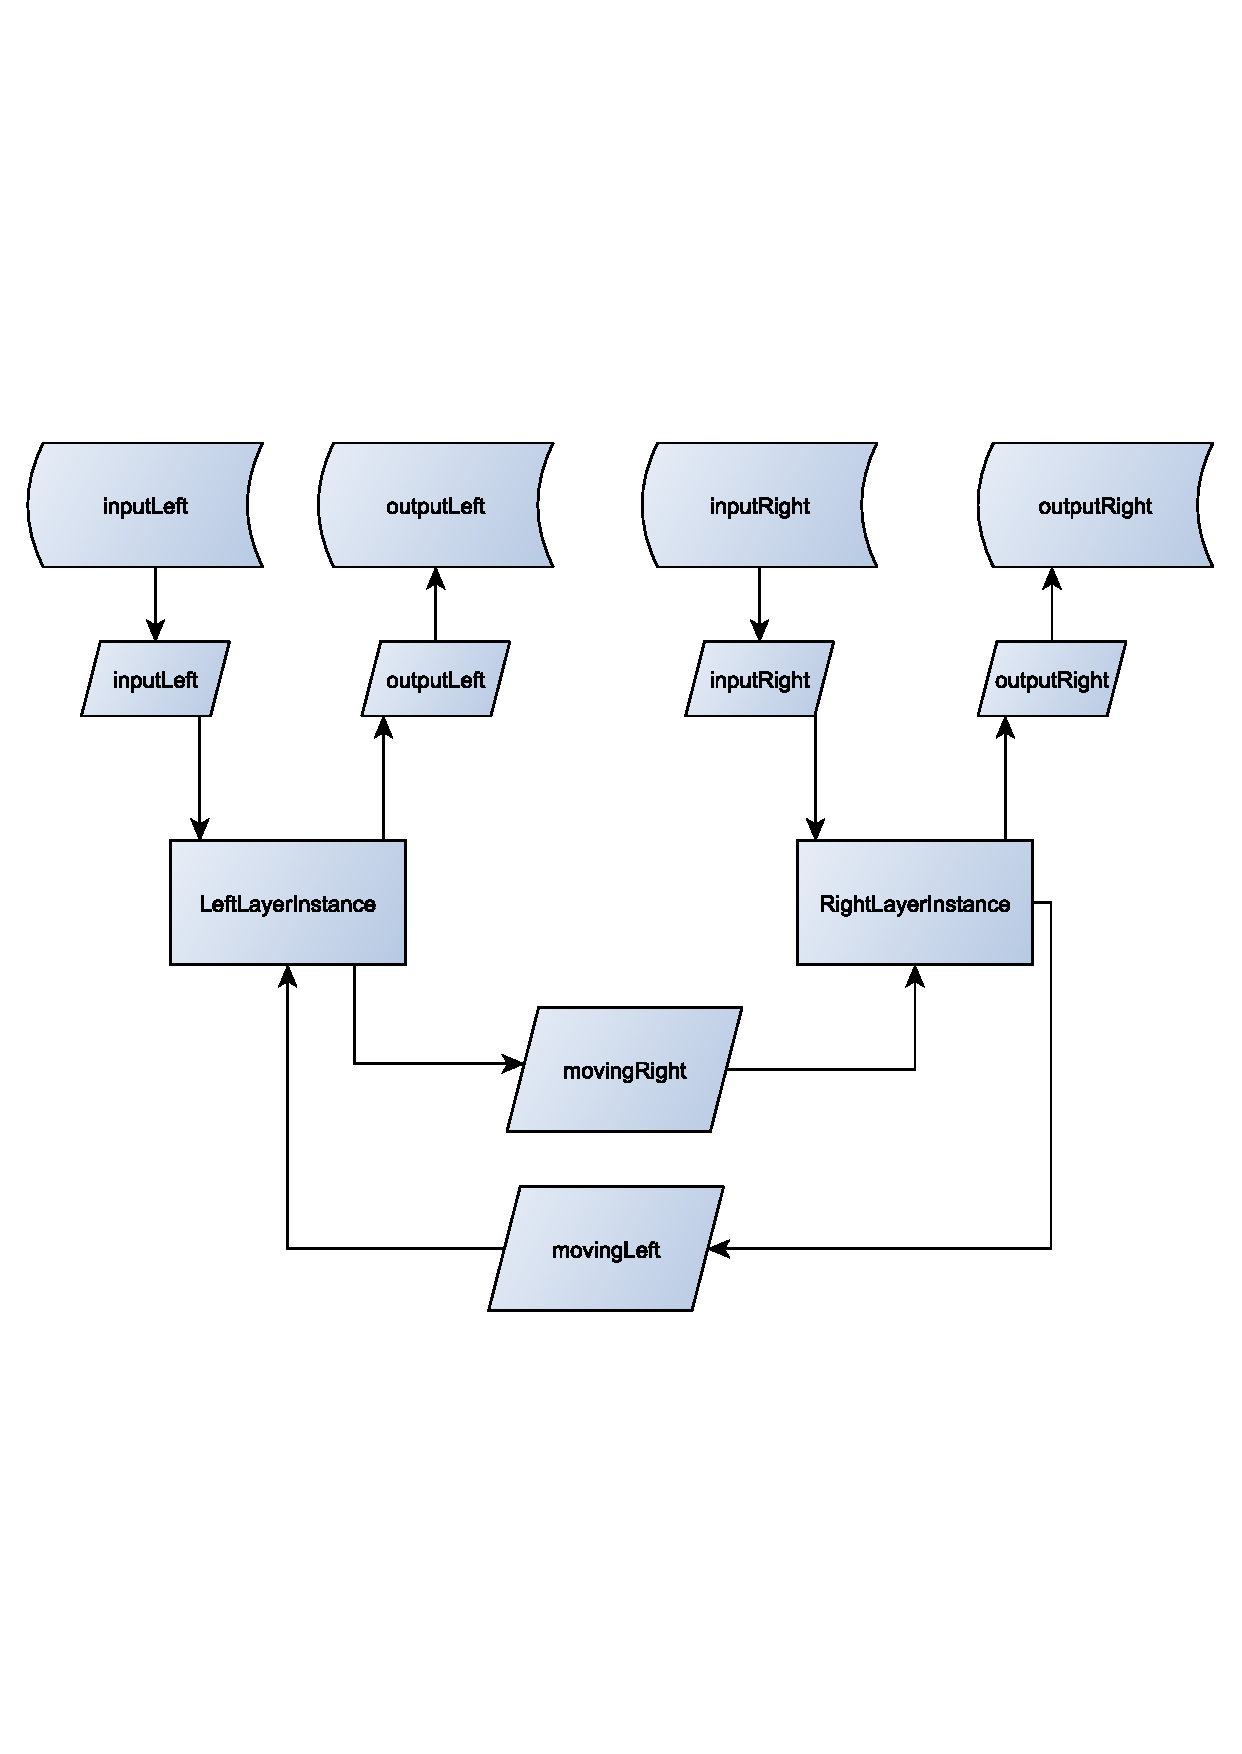
\includegraphics[scale=0.5,trim=0 200 0 200]{twoInstanceTest.pdf}%l b r t
	\caption{Two instances communicating directly trough buffer}
	\label{fig:twoInstanceTest}	
	\end{center}
\end{figure}



\section{Creating a test program}
In the beginning one simply includes the layer and in the function sets the name of the layer. It's is possible to change the defined names for the .dat files. The boost buffers are defined for the layer, so with this setup it's just running the program.
Figure \ref{fig:TestFlowchart} shows the flowchart testing a single layer by feeding input to the inputbuffer, and after initiating the layer, collecting the output from the outputbuffer. 


\begin{figure}[htb]
	\begin{center}
	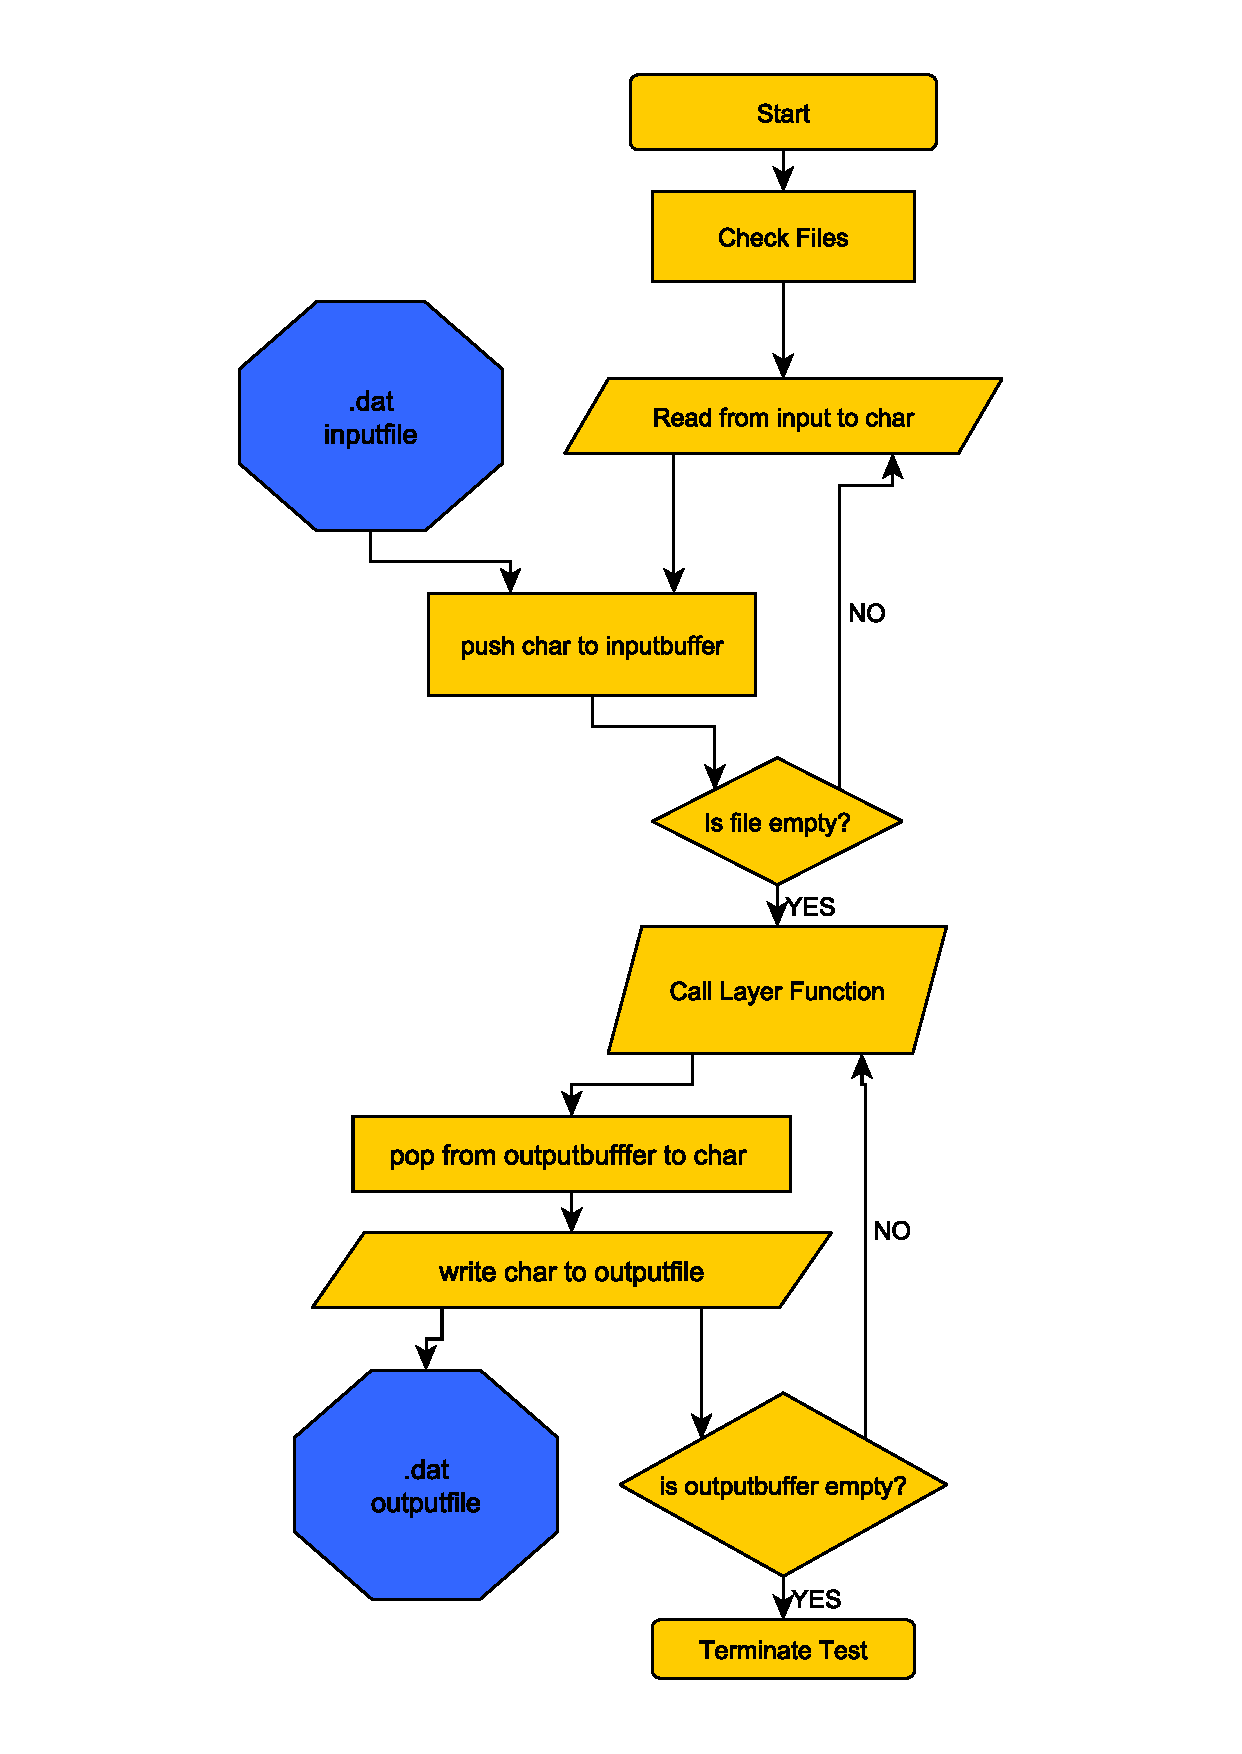
\includegraphics[scale=0.5,trim=0 10 0 10]{TestFlowchart.pdf}
	\caption{Flowchart for test function, testing a single direction}
	\label{fig:TestFlowchart}	
	\end{center}
\end{figure}

\subsection{Physical Layer}

The single instance test, whether the computer is able to send and receive sound have already been done while developing and debugging the layer. Therefore it is more logical to perform a test with two instances of the layer, examining how many of the sent messages are actually received by the other instance.

\subsection{Data link Layer}


The data link Layers main responsibilities is keeping track of the token giving permission to send and framing the messages before they are sent.
To test that the framing are done properly, a test of a single instance of the data link layer is done. The two instance test is used for two purposes; testing the token and the ability to communicate with errors. The token test is mostly a debugging issue, but can also be used for optimization.

Testing the ability to communicate with errors is done by having to instances communicate, while inflicting a specified percent of errors. Thus it is possible to test the layers ability to maintain a connection with errors.


\subsection{Transport Layer}

More nEeded!

The transport layer is responsible verifying the checksum. An appropriate test is sending a stream of messages to the transport layer, to see if only the correctly checksummed messages arrive. With the two instance test it would be possible to see if the transport layer is able produce and interpret the checksum.

\subsection{Application Layer}

The application layer is the users program interface. It is able to easily receive data as input and forward it to the transport layer so that it can be sent. A lot of single instance testing and debugging have to done to make sure that the application layer is able to handle all input correct. It is also necessary to create a program mimicking a users program, to test the application layers ability to transfer a file, using the application layers built-in functions. 

The performance of the application layer is tested by building a file transfer program with the application layer recording the speed of transferring the files trough the application layer.

\subsection{Layers Combined}

In this test all the layers are connected and controlled by the backbone. This test is done as a potential user, with the options provided by the application layer. Using the file transfer program from the application layer, it is now tested by sending the file from the application layer test between two computers. 

